\documentclass[11pt]{article}

\usepackage{graphicx}
\usepackage{url}
\newcommand{\numpy}{{\tt numpy}}    % tt font for numpy
\topmargin -.75in
\textheight 9in
\oddsidemargin -.25in
\evensidemargin -.25in
\textwidth 7in

\begin{document}

% https://moodle.up.pt/mod/assign/view.php?id=72723
\author{Miguel Sozinho Ramalho, UP201403027}
\date{June $18^{th}$, 2019}
\title{Algorithms for Bioinformatics: Project 3\\Python module for Automatic Sequence Analysis}
\maketitle

% \medskip

\section{Introduction}
The current report describes the architecture and underlying concepts of a Python3 module whose purpose is the implementation of a \textit{bioinformatics} pipeline. The module should be able to handle biological sequences, perform BLAST\footnote{\url{https://blast.ncbi.nlm.nih.gov/Blast.cgi}} operations on a FASTA\footnote{\url{https://en.wikipedia.org/wiki/FASTA}} database, calculate the result of Multiple Sequences Alignment (MSA), produce distance matrices between a list of biological sequences and use this matrix to perform Unweighted Pair Group Method with Arithmetic mean (UPGMA\footnote{\url{https://en.wikipedia.org/wiki/UPGMA}}) clustering and generate phylogenetic trees, and also produce draw and unweighted graphs from those distance matrices by specifying a maximum distance threshold for two sequences (that ultimately represent a species) to be connected. 

This module is a new version of the previous practical work and so all the base concepts of biological sequences and the base functionality of reading/handling them is assumed to be common ground upon which the new version has been built, as well as the Dynamic Programming techniques used to produce global and local alignments. 

A Jupyter Notebook (run\_me.ipynb) was created to exemplify the use of the developed functionality (a static version is available as run\_me.html) along with unit tests that guarantee the correctness of the software through time and horizontal changes. Documentation was also made and is available in the \textit{docs} folder (open the \textit{docs/\_build/html/index.html} file  or type \textbf{help(bioseq.moduleName)} after installation). 
% Contextualizar e descrever brevemente o problema.

\section{Implementation and Results}
This project was particularly challenging due to a concern for simple and fast implementation for algorithms, such as the UPGMA. The visualisation of phylogenetic trees and distance graphs was also a novelty and required the use of some new libraries (Phylo\footnote{\url{https://biopython.org/wiki/Phylo}} and Networkx\footnote{\url{https://networkx.github.io/}}). It should be noted that all external libraries used are included in the requirements.txt file which can be used to prepare the python environment with the command \textbf{pip install -r requirements.txt}. TQDM\footnote{\url{https://github.com/tqdm/tqdm}} was used to provide progress bar feedback in typically long operations. Some further considerations for each building block of the pipeline are included below:

\subsubsection{BLASTA}
\begin{itemize}
    \itemsep0em
    \item The database can be loaded from a FASTA file
    \item When performing the search, sequences matching the query (same species) are discarded
    \item A "blast" object can be built with a given database and then reused so that the process of building the database is not executed every time a search must be done
    \item The process of expanding the matching subsequences is done first forward and then backward without code duplication as the backward steps are done forward on the reversed sequences
    \item A custom threshold can be specified (instead of the static "half" rule) to stop the expanding process
    \item All sequences in the database are scored against the query and then the top n are returned (by default n is 10), this is considered to be better than an iterative search of the best match (which inevitably has to score all functions in each iteration)
    \item The score used between sequences was that of the ratio of matches instead of the number of matches, as pragmatically this led to a better result segregation
\end{itemize}

\subsection{MSA}
\begin{itemize}
    \itemsep0em
    \item For cases where the global alignment returns multiple results only the first is considered, this was not considered harmful for the results as the other alignments had the same score and because there is no a priori manner of knowing which alignment is better (time constraints and result interpretation complexity also motivated this decision)
\end{itemize}

\subsection{Phylogenetic Trees (ptrees)}
\begin{itemize}
    \itemsep0em
    \item The input for the ptree generation can either be previously aligned sequences or not yet aligned ones, using the same function call (this is automatically detected)
    \item The Phylo module is used to display the ASCII version of the ptrees as well as the visual ones. This required the implementation of a method that would convert our ptrees into an XML version that Phylo could read\footnote{\url{https://biopython.org/wiki/PhyloXML}}, but that can also useful for other applications
\end{itemize}



\section{Results}
As apendix, there are some pictures outlying the pipeline blocks that are considered interesting or relevant for demonstration purposes. All the used parameters are dynamic so only their default values are included (no default makes sense for the cut value but these can be seen in the run\_me instance [.py, .html, .ipynb]) in Table \ref{tab:parameters}. 


% Deve indicar que funcionalidades foram implementadas, se conseguiu implementar todas as funcionalidades pedidas e se implementou outras funcionalidades além das especificadas.

\section{Conclusions}
All the initial goals were met and a lot was learned both from a bioinformatics perspective as well as algorithmic and knowledge on available libraries. 
% Comentários e Conclusões.

% \section{References}
%  (precisam ser explicitamente citadas no texto para saberem de onde o texto foi retirado/adaptado! Copiar é crime e poderá transformar-se em processo disciplinar, portanto evitem copiar textos e códigos. Se utilizarem figuras retiradas da web ou de livros ou de artigos etc, é necessário colocar uma referência explícita e clara. Por favor tenham atenção aos erros ortográficos.

\begin{table}[h!]
\centering
\begin{tabular}{|c|c|c|c|}
\hline
\textbf{Section} & \textbf{Parameter} & \textbf{Default Value} & \textbf{Details}                        \\ \hline
Blast            & top                & 10                     & how many to return                      \\ \hline
Blast            & threshold          & 0.5                    & when to stop expanding subsequence      \\ \hline
Graph            & cut                & NA                     & include only distances below this value \\ \hline
\end{tabular}
\caption{Parameter default values\label{tab:parameters}}
\end{table}

\newpage

\section*{Appendix}
\appendix 

\begin{figure}[h!]
    \centering
    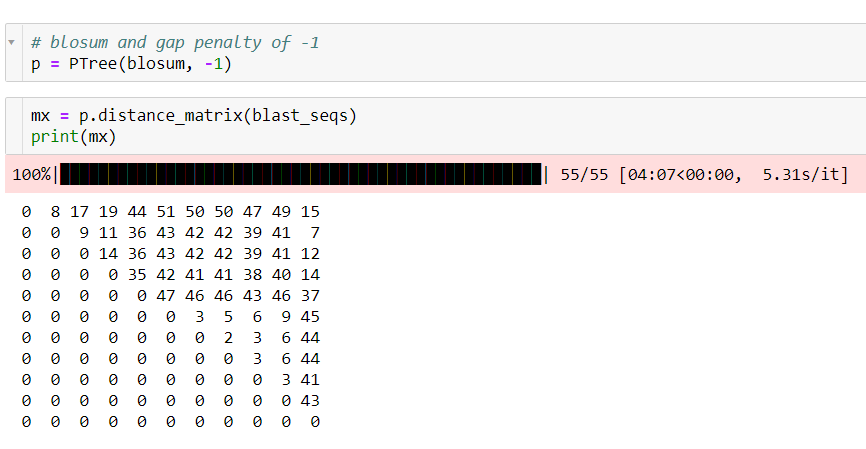
\includegraphics{matrix.png}
    \caption{Distance Matrix}
\end{figure}

\begin{figure}[h!]
    \centering
    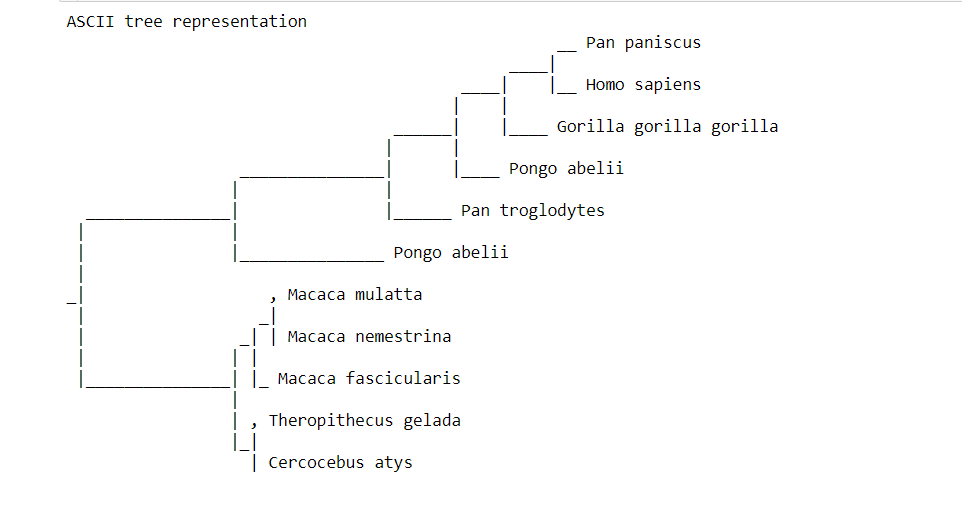
\includegraphics{tree_ascii.png}
    \caption{ASCII output of the phylogenetic tree}
\end{figure}

\begin{figure}[h!]
    \centering
    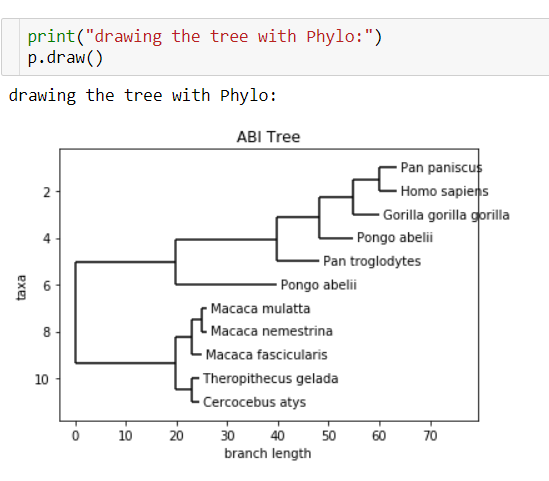
\includegraphics{image_tree.png}
    \caption{Dynamic visualization of a phylogenetic tree}
\end{figure}

\begin{figure}[h!]
    \centering
    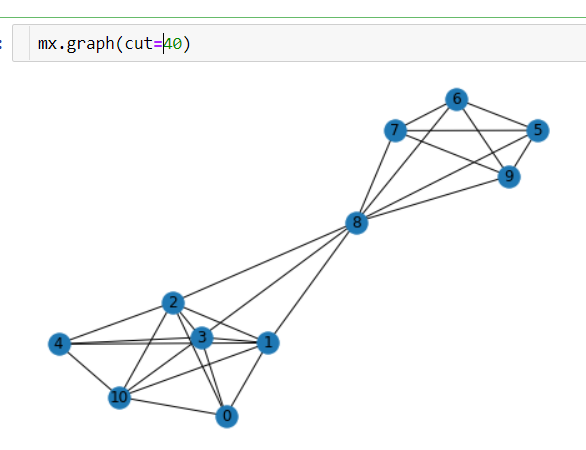
\includegraphics{graph.png}
    \caption{Example of one of the generated graphs}
    \label{fig:my_label}
\end{figure}

\end{document}
\grid
\grid